\section{Theorie}
Ein Hohlleiter ist ein Metallrohr, indem Energie transportiert werden kann.
In diesem Versuch wird ein rechteckiger Hohlleiter verwendet, es gibt aber
auch elliptische oder runde Hohlleiter.

In einem Hohlleiter können
elektromagnetische Schwingungen in verschiedenen Moden weitergeleitet werden.
Jeder Modus besitzt eine Cut-Off-Frequenz, welche durch die Abmessung des
Hohlleiters bestimmt wird. Unter dieser Frequenz kann keine Energie
weitergeleitet werden.
Es wird zwischen zwei Moden unterschieden: der "transversal elektrischen"
(TE-Modus) und der "transversal magnetischen" (TM-Modus) Mode. Hierbei steht das
jeweilige Feld überall senkrecht auf der Ausbreitungsrichtung bzw. der
Hohlleiterachse. Ein Spezialfall ist die Überlagerung beider Moden: Bei dem
TEM-Modus steht sowohl das magnetische als auch das elektrische Feld senkrecht
zur Ausbreitungsrichtung (wie bei einer freien elektromagnetischen Welle oder
einem Koaxialleiter). Die Indizes an dem Modus beschreiben die Anzahl der
Halbwellen des Feldes in die zwei Hauptrichtungen. Als Beispiel ist in Abbildung
\ref{abb:1} der $\text{TE}_{\symup{1,0}}$-Modus in einem rechteckigen Hohlleiter
zu sehen.

\begin{figure}
  \centering
  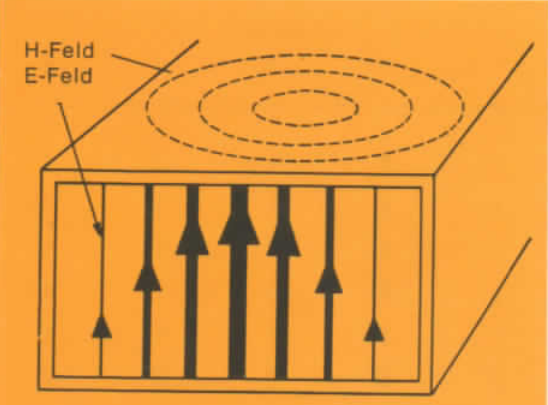
\includegraphics[scale=0.25]{Mode_1_0.png}
  \caption{$\text{TE}_{\symup{1,0}}$-Modus in einem rechteckigen Hohlleiter.
  \cite{Q1}}
  \label{abb:1}
\end{figure}

In Abbildung \ref{abb:2} ist das Blockschaltbild eines Klystron zu sehen.
Ein Klystron ist eine Mikrowellenröhre, bei der aus einem kontinuierlichen
Elektronenstrahl mittels Geschwindigkeitsmodulation Mikrowellenenergie gewonnen
wird. Hierbei werden Elektronen aus der Kathode emittiert und in Richtung der
Gitter beschleunigt.
Aufgrund der Fermi-Dirac-Verteilung besitzen die Elektronen unterschiedliche
Anfangsgeschwindigkeiten, wenn diese aus der Kathode austreten. Der Reflektor
hat gegenüber der Kathode ein negatives Potential, sodass die Elektronen
reflektiert werden. Somit durchlaufen die Elektronen erneut das Resonatorgitter.
Durch die unterschiedlichen Geschwindigkeiten der Elektronen, entstehen bei der
Reflexion Bündel aus Elektronen, da schnelle Elektronen näher zur Kathode
gelangen als langsame Elektronen.
Fängt das Klystron nun an zu schwingen, werden die eintretenden Elektronen, je
nach Ausrichtung des elektrischen Feldes, entweder abgebremst oder beschleunigt.
Bei einer Abbremsung geben die Elektronen einen Teil ihrer Energie an den
Resonator ab, das Klystron schwingt. Die stärkste Schwingung tritt bei einer
Verweilzeit im Resonator von $n+\frac{3}{4}$ der Periodendauer auf
($n \in \mathbb{N}$). Bei einer Beschleunigung nehmen die Elektronen Energie
vom Klystron auf und es entsteht keine Schwingung.

\begin{figure}
  \centering
  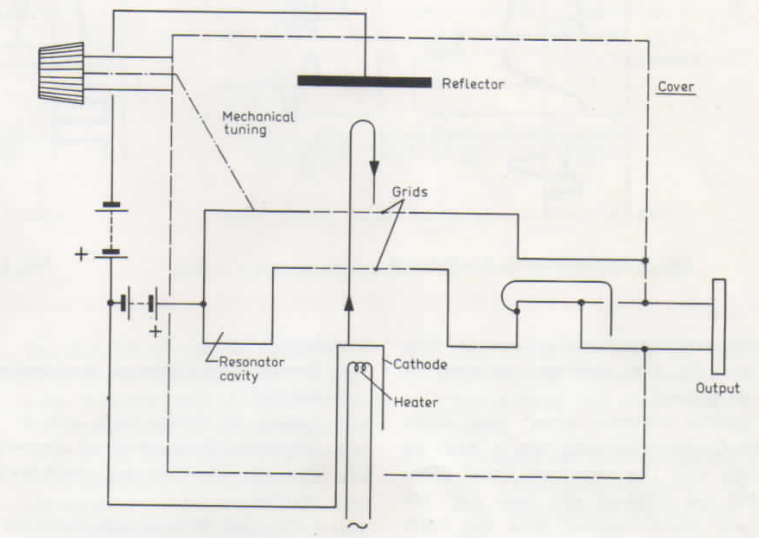
\includegraphics[scale=0.4]{Blockschaltbild.png}
  \caption{Blockschaltbild des Klystrons.\cite{Q1}}
  \label{abb:2}
\end{figure}

In Abbildung \ref{abb:3} sind die Zusammenhänge zwischen Reflektorspannung,
Ausgangsleistung und Schwingungsfrequenz dargestellt. Zu erkennen ist, dass nur
bei bestimmten Reflektorspannungen Schwingen auftreten, da diese von der
Laufzeit der Elektronen abhängt. Diese Schwingen werden auch Moden genannt.
Da die Frequenz direkt von der Abmessung des Resonatorhohlraums abhängt, ist
durch Veränderung des Resonatorvolumens eine \textbf{mechanische Abstimmung} des
Klystrons möglich. Durch Veränderung der Reflektorspannung lässt sich die
Frequenz auch minimal ändern, dies wird \textbf{elektronische Abmessung} genannt.


\begin{figure}
  \centering
  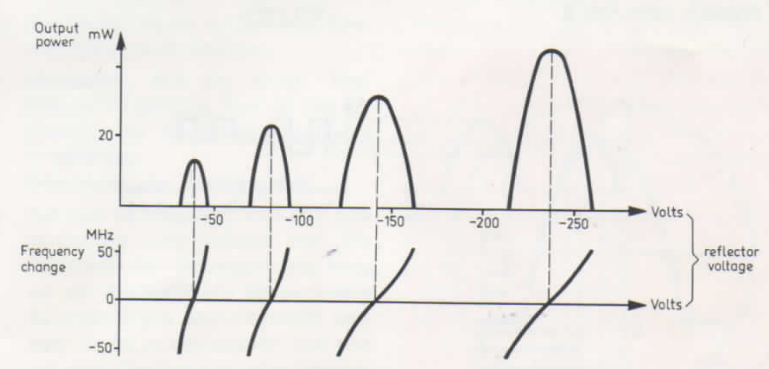
\includegraphics[scale=0.4]{Graph1.png}
  \caption{Zusammenhang zwischen Reflektorspannung, Ausgangsleistung und
  Schwingungsfrequenz. \cite{Q1}}
  \label{abb:3}
\end{figure}

Die Sinusmodulation über die Reflektorspannung ist in Abbildung \ref{abb:4a}
dargestellt.
Falls die Ausgangsleistung über ein SWR-Meter angezeigt werden soll, so muss das
Klystron Amplitudenmoduliert werden. Für eine Rechteckspannung ist dies in
Abbildung \ref{abb:4b} a) dargestellt. In Abbildung \ref{abb:4b} b) ist das
gleiche Ergebnis zu sehen, nur hierbei wurde die Modulationsspannung wie in der
Abbildung zu sehen angelegt. Für die Modulierung ist neben der richtigen
Modulationsspannung auch die richtige Amplitude wichtig.

\begin{figure}
  \centering
  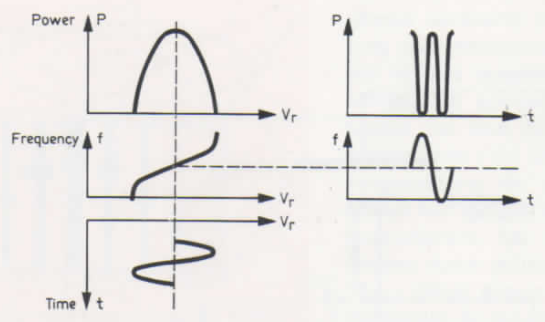
\includegraphics[scale=0.4]{Sinusmodulation.png}
  \caption{Sinusmodulation. \cite{Q1}}
  \label{abb:4a}
\end{figure}
\begin{figure}
  \centering
  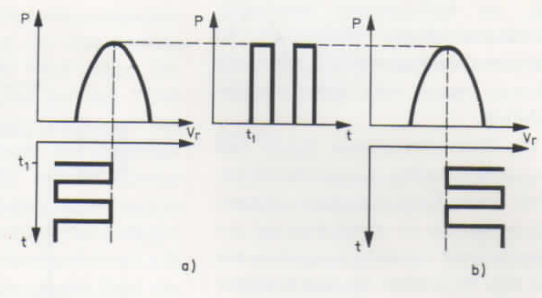
\includegraphics[scale=0.4]{Rechteckmodulation.png}
  \caption{Rechteckmodulation. \cite{Q1}}
  \label{abb:4b}
\end{figure}

\subsection{Frequenz und Wellenlänge}

In einem luftgefüllten Rechteckhohlleiter gilt allgemein für die
$\text{TE}_{\symup{m,n}}$-Mode oder die $\text{TM}_{\symup{m,n}}$-Mode:
\begin{equation}
  \lambda_g =  \frac{\lambda_0}{\sqrt{1-\left(\frac{\lambda_0}{\lambda_c}\right)^2}}
  \label{eq:lambda_g}
\end{equation}
mit
\begin{equation}
  \lambda_c = \frac{2}{\sqrt{\left(\frac{m}{a} \right)^2 + \left(\frac{n}{b} \right)^2}}
  \label{eq:lambda_c}
\end{equation}
($\lambda_0$ Wellenlänge im freien Raum, $\lambda_g$ Wellenlänge im Hohlleiter,
$\lambda_c$ Grenzwellenlänge im Hohlleiter, $a$ Breitseite des Hohlleiters, $b$
Schmalseite des Hohlleiters)

Da ein Hohlleiter meistens in der niedrigsten Mode verwendet wird gilt hier für
die $\text{TE}_{\symup{1,0}}$-Mode oder die $\text{TM}_{\symup{1,0}}$-Mode:
\begin{equation}
  \lambda_c = \frac{2}{\sqrt{\left(\frac{1}{a} \right)^2 + \left(\frac{0}{b} \right)^2}} = 2a
  \label{eq:lambda_c_TE01}
\end{equation}
und damit für die Wellenlänge im Hohlleiter:
\begin{equation}
  \lambda_g =  \frac{1}{\sqrt{1-\left(\frac{\lambda_0}{2a}\right)^2}}
  \label{eq:lambda_g_TE01}
\end{equation}
Mit der Beziehung $f=\frac{c}{\lambda_0}$ folgt für die Frequenz:
\begin{equation}
  f = c \cdot \sqrt{\left(\frac{1}{\lambda_g}\right)^2+\left(\frac{1}{2a}\right)^2}
  \label{eq:Frequenz}
 \end{equation}
 Die Hohlleiterwellenlänge kann durch den doppelten Abstand zwei
 aufeinanderfolgender Minima (oder Maxima) im Stehwellenfeld direkt gemessen werden.
Bei der Grenzfrequenz ist $\lambda_g$ unendlich groß, das bedeutet, dass sich
das Feld entlang des Hohlleiters nicht ändert. Somit kann auch keine Energie
transportiert werden.

\subsection{Dämpfung}
Die Dämpfung wird gewöhnlich in Dezibel angegeben:
\begin{equation}
  \left(\frac{P_1}{P_2}\right)_{\symup{dB}} = 10 \cdot (\log{P_1}-\log{P_2})
\end{equation}
mit dem Leistungsverhältnis $\frac{P_1}{P_2}$.
In diesem Versuch wird ein Semipräzisionsabschwächer verwendet.

\subsection{Stehwellenmessung}
In dem Hohlleiter überlagern sich die einfallende und die reflektierte Welle.
Diese entsteht durch Unstetigkeiten in der Leitung oder durch eine Lastimpedanz.
Haben beide Wellen die gleiche Phasenlage, entsteht durch die Überlagerung eine
maximale Feldstärke.
Der Spannungs-Reflexionskoeffizient $\rho$ ist definiert als das Verhältnis
zwischen der emittierten und der reflektierten Welle.
Das Spannungs-Schwellen-Verhältnis (SWR) wird durch das Verhältnis der
maximalen und der minimalen Feldstärke der stehenden Welle beschrieben.
Zur Bestimmung der Welligkeiten gibt es mehrere Verfahren:
\begin{itemize}
  \item \textbf{Direkte Messung}: Über eine Sonde (Antenne) kann ein Teil des
  elektrischen Feldes ausgekoppelt werden und auf einem SWR-Meter sichtbar
  gemacht werden. Hierbei darf die Sondentiefe nicht zu groß sein, um das
  elektrische Feld nicht zu sehr zu stören. Die Welligkeit kann direkt an
  dem SWR-Meter abgelesen werden.
  \item \textbf{3dB-Methode}: Hierbei wird der Abstand zwischen zwei Punkten ($d_1-d_2$)
  gemessen, an denen die Detektorspannung das doppelte des Minimums beträgt.
  \begin{equation}
    S= \sqrt{a+\frac{1}{\left(\sin{\frac{\pi(d_1-d_2)}{\lambda_g}}\right)^2}}
    \approx \frac{\lambda_g}{\pi (d_1-d_2)}
    \label{eq:3dB}
  \end{equation}
  Die Näherung in gilt für $S>10$.
  \item \textbf{Abschwächer-Methode}: Das Ausgangssignal des Detektors im Maximum
  wird dem Signal im Minimum mit Hilfe des Abschwächers gleichgemacht. Aus der
  Differenz des Abschwächers lässt sich das SWR berechnen:
  \begin{equation}
    A_2-A_1 = 20 \log{S}
    \label{eq:Abschwaechermethode}
  \end{equation}
\end{itemize}

\section{Durchführung}

\subsection{Untersuchung des Reflexklystrons}

Der Versuch wird wie in Abbildung \ref{abb:Aufbau1} zu sehen aufgebaut.

\FloatBarrier
\begin{figure}
  \centering
  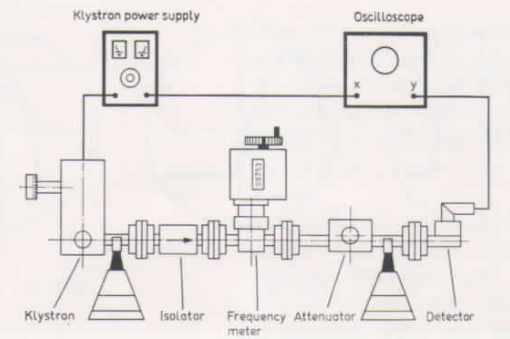
\includegraphics[scale=0.5]{Aufbau1.png}
  \caption{Aufbau zur Untersuchung des Klystrons. \cite{Q1}}
  \label{abb:Aufbau1}
\end{figure}
\FloatBarrier

Das Dämpfungsglied wird auf \SI{40}{\dB}. Die Amplitude der Sinusspannung wird so
eingestellt, dass sich eine horizontale Linie parallel zur Mittellinie ergibt.
Die Reflektorspannung wird auf etwa \SI{200}{\volt} eingestellt, diese wird
so lange variiert, bis die Modenkurve im Mittelpunkt des Oszilloskopes liegt
(siehe Abbildung \ref{abb:Versuch1.1}).
Der Frequenzmesser wird so abgestimmt, dass eine Sattelung an der Spitze der
Modenkurve entsteht. Dabei soll die Frequenz bei etwa \SI{9}{\giga\hertz} liegen.
Weicht die Frequenz zu sehr von dem Wert ab, muss die Amplitude der Sinusspannung
oder der Abstimmknopf des Klystrons variiert werden, sodass
bei einer Frequenz von \SI{9}{\giga\hertz} die gewünschte Sattelung entsteht
(siehe Abbildung \ref{abb:Versuch1.2}).
Die Frequenz und die Resonatorspannung wird abgelesen.
Den Frequenzmesser verstimmen, sodass keine Sattelung mehr vorhanden ist und die
Amplitude ablesen. Die Reflektorspannung so einstellen, dass der Rand der
Modenkurve in der Mitte des Oszilloskops liegt wie in Abbildung
\ref{abb:Versuch1.3} und die Reflektorspannung ablesen. Das gleiche mit der
anderen Seite der Mode durchführen.

\FloatBarrier
\begin{figure}
  \centering
  \begin{subfigure}{0.2\textwidth}
    \raggedleft
    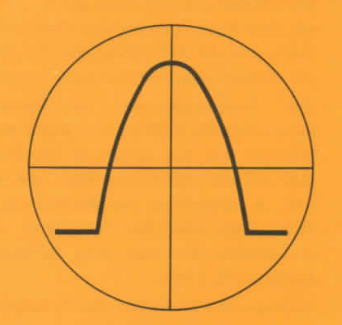
\includegraphics[width=0.93\textwidth]{Versuch1.1.png}
    \caption{}
    \label{abb:Versuch1.1}
  \end{subfigure}
  \begin{subfigure}{0.2\textwidth}
    \centering
    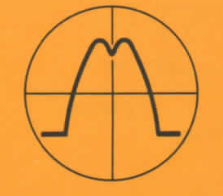
\includegraphics[width=\textwidth]{Versuch1.2.png}
    \caption{mit Sattelung}
    \label{abb:Versuch1.2}
  \end{subfigure}
  \begin{subfigure}{0.2\textwidth}
    \raggedright
    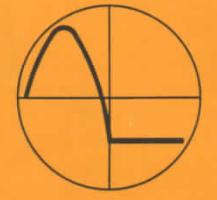
\includegraphics[width=0.955\textwidth]{Versuch1.3.png}
    \caption{Breitenmessung}
    \label{abb:Versuch1.3}
  \end{subfigure}
  \caption{Modenkurven.\cite{Q1}}
\end{figure}
\FloatBarrier

Für die elektronische Abstimmung wird die Reflektorspannung so moduliert, dass
die Sattelung erneut erreicht wird. Die Frequenz und die Reflektorspannung wird
notiert. Die Frequenz wird so variiert, das die Modenkurve auf dem Oszilloskop
der Modenkurve in den Abbildungen \ref{abb:Versuch1.4} und \ref{abb:Versuch1.5}
gleicht. Auch hier wird jeweils die Frequenz und die Reflektorspannung notiert.

\begin{figure}
  \centering
  \begin{subfigure}{0.3\textwidth}
    \raggedleft
    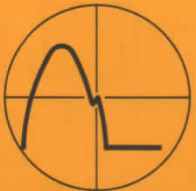
\includegraphics[width=0.58\textwidth]{Versuch1.4.png}
    \caption{}
    \label{abb:Versuch1.4}
  \end{subfigure}
  \begin{subfigure}{0.3\textwidth}
    \raggedright
    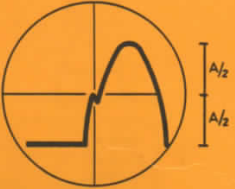
\includegraphics[width=0.7\textwidth]{Versuch1.5.png}
    \caption{}
    \label{abb:Versuch1.5}
  \end{subfigure}
  \caption{Modenkurven elektronische Abstimmung.\cite{Q1}}
\end{figure}

\subsection{Messung von Frequenz, Wellenlänge und Dämpfung}

Der Versuch wird nach Abbildung \ref{abb:Versuch2.Aufbau} umgebaut.

\FloatBarrier
\begin{figure}
   \centering
  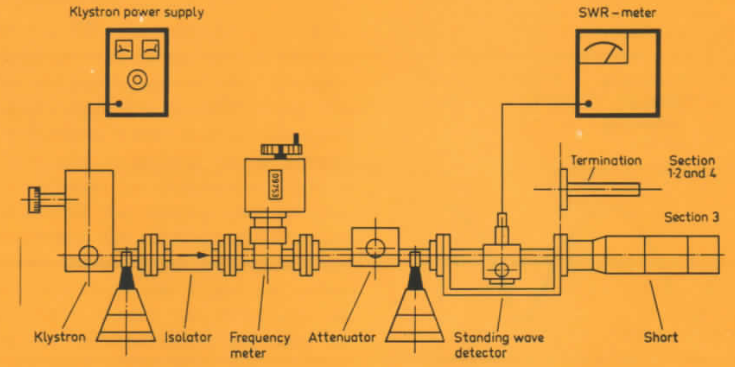
\includegraphics[scale=0.3]{Versuch2.Aufbau.png}
  \caption{Aufbau zur Messung der Frequenz, Wellenlänge und Dämpfung. \cite{Q1}}
  \label{abb:Versuch2.Aufbau}
\end{figure}
\FloatBarrier

Das Dämpfungsglied wird auf \SI{20}{\dB} und die Reflektorspannung auf etwa
\SI{200}{\volt} eingestellt. Am SWR-Meter werden \SI{40}{\dB} und eine Bandbreite von
\SI{100}{\hertz} eingestellt. Mit Hilfe des \SI{1}{\kilo\hertz}-Reglers einen
maximalen Ausschlag erzeugen.

Für die direkte Frequenzmessung den Frequenzmesser modulieren, bis ein Minimum
auf dem SWR-Meter zu erkennen ist. Die Frequenz notieren.

Den festen Abschluss durch den verstellbaren Abschluss ersetzen und den
Frequenzmesser verstimmen. Es werden nun mit Hilfe der Sonde die Punkte
minimalen Ausschlags gesucht und notiert.

Zur Messung der Dämpfung wird erneut der feste Abschluss montiert und der
Frequenzmesser auf \SI{9000}{\kilo\hertz} eingestellt. Die Verstärkung des
SWR-Meters wird so variiert, bis ein Maximum auf dem SWR-Meter zu erkennen ist.
Das Dämpfungsglied wird so eingestellt, sodass die Dämpfung bei \SI{0}{\dB}
liegt. Die Mikrometeranzeige ablesen und notieren. Den Vorgang bis \SI{10}{\dB}
in \SI{2}{\dB}-Schritten wiederholen.

\subsection{Stehwellen-Messungen}

Für den letzten Versuchsteil wird der Versuchsaufbau nach Abbildung
\ref{abb:Versuch3.Aufbau} verändert.

\FloatBarrier
\begin{figure}
  \centering
  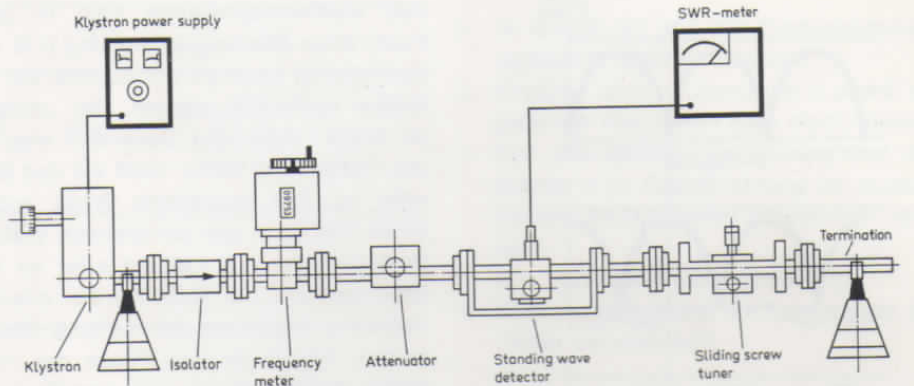
\includegraphics[scale=0.3]{Versuch3.Aufbau.png}
  \caption{Aufbau Stehwellen-Messungen. \cite{Q1}}
  \label{abb:Versuch3.Aufbau}
\end{figure}
\FloatBarrier

Der Abschwächer wird auf \SI{20}{\dB} eingestellt. Am SWR-Meter wird die
Bandbreite auf \SI{20}{\hertz} umgestellt und der \SI{40}{\dB}-Knopf gedrückt.
Die Sonde zur Messung der Feldstärke wird auf Höhe der roten Linie festgeschraubt.
Die Sonde des Gleitschraubentransformators wird ganz herausgedreht.
Das Klystron wird mit \SI{9000}{\kilo\hertz} und einer Rechteckmodulation
(\SI{1000}{\hertz}) zum Schwingen gebracht.

Zur Messung der kleinen und mittleren Welligkeiten die Sondentiefe des
Gleitschraubentransformators auf 3, 5, 7 und 9\,mm einstellen und jeweils ein
Minimum und ein Maximum  durch Verschieben der Messsonde suchen und die Abstände
notieren.

Bei der "\SI{3}{\dB}-Methode" werden nun große Welligkeiten gemessen. Die Sonde
des Gleitschraubentransformators wird auf \SI{9}{\milli\meter} gestellt und es
wird erneut ein Minimum mittels der Messsonde gesucht. Mit Hilfe des Verstärkers
am SWR-Meter wird die Anzeige auf \SI{3}{\dB} verstellt. Die Messsonde wird nun
nach links verschoben, bis die Anzeige des SWR-Meters \SI{0}{\dB} anzeigt und
die Position der Messsonde ablesen. Das gleiche wird erneut durchgeführt, nur dass
die Messsonde nach rechts verschoben wird.

Den Gleitschraubentransformator und den veränderbaren Abschluss durch den
festen Abschluss ersetzen. Mittels der Messsonde den Abstand zwei
aufeinanderfolgender Minima ausmessen.

Zuletzt wird die Abschwächer-Methode durchgeführt:
Erneut den Gleitschraubentransformator und den festen Abschluss in den
Versuchsaufbau einfügen. Die Sondentiefe des Gleitschraubentransformator auf
\SI{9}{\milli\meter} einstellen und die Messsonde in ein Minimum verschieben.
Das Dämpfungsglied auf $A_1=\SI{20}{\dB}$ und die Verstärkung des SWR-Meters
einstellen, sodass der Ausschlag bei \SI{3}{\dB} liegt. Durch Veränderung des
Dämpfungsglieds bei Verschieben der Messleitung wird das relative Maximum
bestimmt.

\section{Auswertung}

\subsection{Vermessung der Moden}
Zur Untersuchung dreier Moden werden jeweils die Reflektorspannungen an den rechten ($U_2$)
und linken Nullstellen ($U_1$), sowie im Maximum ($U_0$) ermittelt.
Die Ergebnisse sind gemeinsam mit den Amplituden der drei Moden in Tabelle
\ref{tab:Moden} zu sehen. In Abbildung \ref{fig:Moden} sind die Messwerte graphisch
zusammen mit den angedeuteten Modenkurven abgebildet.
\FloatBarrier
\begin{table}
    \centering
    \begin{tabular}{c c c c c c}
        \toprule
        {Mode} & {Reflektorsp.} & {Reflektorsp.} & {Reflektorsp.} & {Amplitude} & {Frequenz} \\
        {}     & {$U_0$ \,/\,$\si{V}$} & {$U_1$ \,/\,$\si{V}$} & {$U_2$ \,/\,$\si{V}$} & {$A$ \,/\,$\si{V}$ } & {$f_0$\, / \, $\si{MHz}$} \\
        \midrule
        Mode 1  &  215  &  200  &  230  &  0,124  &  9000     \\
        Mode 2  &  135  &  120  &  150  &  0,134  &  9005     \\
        Mode 3  &   80  &   70  &   90  &  0,108  &  9010     \\
        \bottomrule
    \end{tabular}
    \caption{Messwerte für die Reflektorspannungen, bei denen jeweils die rechte und linke Nullstelle, sowie das Maximum
    auf dem Referenzpunkt im Oszillographen lagen und die zugehörigen Amplituden und Frequenzen.}
    \label{tab:Moden}
\end{table}
\FloatBarrier

\noindent Die Messwerte können durch eine Funktion folgender Form gefittet werden, um die
Modenkurven graphisch darzustellen:
\begin{align*}
    A(U) = x \cdot U^2 + y \cdot U + z \; .
\end{align*}

\noindent Die Fitparameter, die sich für die drei Moden ergeben, sind in Tabelle
\ref{tab:Modenfit} zu sehen. Da die Fitfunktion eine Parabel darstellt und ledigleich
drei Messwerte genommen werden, können keine Fehler angegeben werden, da sich eine
Parabel stets fehlerfrei durch drei Punkte legen lässt.
\FloatBarrier
\begin{table}
    \centering
    \begin{tabular}{c c c c}
        \toprule
            {}    &  {Paramter x}  &  {Parameter y } &  {Paramter  z }\\
        \midrule
        Mode 1 &  -0,00055  &  0,23698  &  -25,35111          \\
        Mode 2 &  -0,00060  &  0.16080  &  -10,72000          \\
        Mode 3 &  -0.00108  &  0.17280  &  -6.804000          \\
        \bottomrule
    \end{tabular}
    \caption{Fitparamter zur Erstellung des Plots \ref{fig:Moden}.}
    \label{tab:Modenfit}
\end{table}
\FloatBarrier
\begin{figure}
  \centering
  \includegraphics[width = 12 cm]{moden.pdf}
  \caption{Graphen der drei Moden.}
  \label{fig:Moden}
\end{figure}
Die Reflektorspannungen und Frequenzen, bei denen sich im Oszilloskop ein Einsattelung
im Maximun, sowie auf der linken oder rechten Flanke der Mode ergaben, sind in Tabelle
\ref{tab:elektronische_Abstimmung} zu sehen.
\FloatBarrier
\begin{table}
    \centering
    \begin{tabular}{c c c c}
        \toprule
        {}    & {Einsattelung auf Max.} & { Einsattelung re. } & {Einsattelung li.} \\
        \midrule
        Reflektorspannung / $\si{\V}$ & 215 & 205 & 225                           \\
        Frequenz / $\si{\MHz}$ & 9000 & 8983 & 9021                               \\
        \bottomrule
    \end{tabular}
    \caption{Messwerte zur elektronischen Abstimmung des Klystrons.}
    \label{tab:elektronische_Abstimmung}
\end{table}
\FloatBarrier
Die Bandbreite $\Delta f_{E}$ wird mit folgender Formel berechnet:
\begin{align*}
    \Delta f_E = f^{\prime\prime} - f^{\prime}
\end{align*}
\FloatBarrier
und beträgt $\SI{38}{MHz}$.
Daraus lässt sich nun die Abstimmempfindlichkeit $E$ mittels folgender Formel berechnen:
\begin{align*}
    E &= \frac{\Delta f_{E}}{V^{\prime \prime}-V^{\prime}} \\
      &= \SI{1,9}{\MHz \per \V} \;.
\end{align*}

\subsection{Messung von Frequenz, Wellenlänge und Dämpfung}
Zur Bestimmung der Wellenlänge im Hohlleiter wurde die Lage zweier aufeinander
folgende Minima, sowie die eingestellte Frequenz aufgenommen. Die Werte finden
sich in Tabelle \ref{tab:Frequenz}. Der doppelte Abstand der Minima entspricht dabei
der Hohlleiterwellenlänge ($\lambda_{g}$) und ergibt sich mit den aufegnommenen Messwerten zu:
\begin{align*}
    \lambda_{g} = \SI{58}{\mm}
\end{align*}
\begin{table}
    \centering
    \begin{tabular}{c c c}
        \toprule
        {Frequenz / $\si{\MHz}$ } & {1. Minimum / $\si{\mm}$ } & { 2. Minimum / $\si{\mm}$} \\
        \midrule
        9010   &  84  &  55  \\
        \bottomrule
    \end{tabular}
    \caption{Messwerte zweier aufeinander folgender Minima und zugehöriger Frequenz.}
    \label{tab:Frequenz}
\end{table}
Mit Hilfe der Gleichung \ref{eq:Frequenz} und der Angabe für die Länge der Längsseite
des Hohlleiters ($a = \SI{22,860(46)}{\mm}$) aus der Versuchsanleitung \cite{Q1} lässt
sich die Frequenz im Hohlleiter berechnen:
\begin{align*}
    f = \SI{8355(10)}{\MHz} \; .
\end{align*}
\\
Die aufegnommenen Werte für die Dämpfung, die zugehörige Mikrometereinstellung,
sowie die aus der Eichkurve abgelesene Dämpfung sind in Tabelle \ref{tab:Daempfung}
zu sehen.
\FloatBarrier
\begin{table}
    \centering
    \begin{tabular}{c c c }
        \toprule
        {SWR-Meter Ausschlag / $\si{\dB}$ } & { Mikrometereinstellung / $\si{\mm}$} & {Dämpfung aus Eichkurve / $\si{\dB}$ } \\
        \midrule
         0       &       3,38        &       22      \\
         2       &       3,60        &       24      \\
         4       &       3,81        &       26      \\
         6       &       3,98        &       29      \\
         8       &       4,07        &       30      \\
        10       &       4,26        &       33      \\
        \bottomrule
    \end{tabular}
    \caption{Gemessene Werte für die Dämpfung, Mikrometereinstellung, sowie abgelesene, zugehörige Werte aus der Eichkurve.}
    \label{tab:Daempfung}
\end{table}

\noindent Die graphische Darstellung der gemessenen Dämpfungswerte, sowie die Eichkurve ist in
Abbildung \ref{fig:Daempfung} zu sehen.
\FloatBarrier
\begin{figure}
    \centering
    \includegraphics[width = 12 cm]{Daempfung.pdf}
    \caption{Eichkurve und gemessene Werte für die Dämpfung.}
    \label{fig:Daempfung}
\end{figure}
\FloatBarrier

\subsection{Bestimmung des Stehwellenverhältnisses}
In Tabelle \ref{tab:SWR_Methode} sind die am SWR-Meter gemessenen Ausschläge für
das Stehwellenverhältnis in Abhängigkeit der Sondentiefe am Gleitschraubentransformator
zu sehen.
\FloatBarrier
\begin{table}
    \centering
    \begin{tabular}{c c}
        \toprule
        {SWR-Meter Ausschlag / $\si{\dB}$} & Sondentiefe / $\si{\mm}$ \\
        \midrule
        1,02    &   3       \\
        1,06    &   5       \\
        1,55    &   7       \\
        4,0     &   1,55    \\
        \bottomrule
    \end{tabular}
    \caption{Messwerte für die SWR-Methode.}
    \label{tab:SWR_Methode}
\end{table}
\FloatBarrier
Tabelle \ref{tab:3dB_Methode} zeigt die Messwerte, die zur Bestimmung des Stehwellenverhältnisses
mittels der 3dB Methode aufgenommen wurden. Aus der Lage der beiden Minima lässt sich zunächst
die Wellenlänge $\lambda_{g}$ berechnen. Mit Hilfe von Formel \ref{eq:3dB} lässt sich dann
das Stehwellenverhältnis berechnen.
\FloatBarrier
\begin{table}
    \centering
    \begin{tabular}{c c c c c c}
        \toprule
        {$d_1$\,/\,mm} & {$d_2$\,/\,mm} & {1. Minimum\,/\,mm} & {2. Minimum\,/\,mm} & {$\lambda_g$ / } & {Stehwellenverhältnis $S$}\\
        \midrule
        95,5    &   71,0    &   96,2    &   71,7    &   49    &     0,64 \\
        \bottomrule
    \end{tabular}
    \caption{Messwerte zur Bestimmung des Stehwellenverältnisses mittels 3dB Methode.}
    \label{tab:3dB_Methode}
\end{table}
\FloatBarrier
Bei der letzten Methode zur Bestimmung des Stehwellenverhältnisses wurden die Dämpfungseinstellungen
$A_{1}= \SI{20}{\dB}$ und $A_{2}=\SI{43}{\dB}$ gemessen.
Aus den beiden Parametern ergibt sich nach Gleichung \ref{eq:Abschwaechermethode}
für das Stehwellenverhältnis ein Wert von:
\begin{align*}
    S_{\text{Abschw.}} = \SI{11,5}{} \; .
\end{align*}

\section{Diskussion}
Die im ersten Versuchsteil aufgenommenen Werte für die Reflektorspannung und die Amplituden
zeigen den zu erwartenden Verlauf. Hier sei darauf hingewiesen, dass die Parabeln
lediglich durch drei Messpunkte gefittet wurden, weshalb keine Fehler für die Fitparameter auftauchen.
Entsprechend der Theorie können Moden mit höheren Frequenzen bei niedrigeren Reflektorspannung festgestellt werden.
Die zunächst mit steigender Reflektorspannung größer werdende Amplitude entspricht der Theorie,
nicht so jedoch die dritte Amplitude, die bei höherer Reflektorspannung wieder kleiner wird.

\noindent Bei der Frequenzbestimmung mittels der Wellenlänge im Hohlleiter ($\lambda_{g}$), fällt
eine Abweichung von $\SI{7,27}{\percent}$ auf. Diese kann durch das am Oszilloskop schwierige
Auffinden der beiden Minima erklärt werden. Dennoch kann der experimentell ermittelte Wert als verhältnismäßig genau
eingestuft werden.

\noindent Bei der Betrachtung der mit dem SWR-Meter gemessenen Werte für die Dämpfung
zeigt sich in beiden Kurven ein sehr ähnlicher Verlauf, der sich lediglich in der Größe
der Funktionswerte unterscheidet. Somit kann auch hier davon ausgegangen werden, dass die
Messwerte plausibel sind.

\noindent
Zum Vergleich der drei Methoden zur Bestimmung des Stehwellenverhältnisses, werden die
drei Ergebnisse bei einer Sondentiefe von $\SI{9}{\mm}$ betrachtet:
\begin{align*}
    S_{\text{SWR-Meter}} &= 4,00    \\
    S_{\text{3dB}} &= 0,64          \\
    S_{\text{Abschw.}} &=11,5       \\
\end{align*}
Es fällt auf, dass sich der Wert für die 3dB-Methode extrem stark von den anderen beiden
Werten unterscheidet, weshalb hier davon ausgegangen werden muss, dass ein Fehler bei der Bestimmung der
Minima entstanden sein muss.
Eine Begründung für den großen Wert, der bei der Abschwächermethode entstand, könnte sein,
dass kein Präzisionsabschwächer verwendet wurde. So kam es bei der Lokalisation der 3dB-Punkte zu
abrupten Vollausschlägen am SWR-Meter.

\printbibliography
